

\chapter{추정 (Estimation)}
\label{estimation}
\index{추정 (estimation)}

이번 장에서 사용되는 코드는 {\tt estimation.py}에 있다.
코드를 다운로드하고 작업하는 것에 대한 정보는 ~\ref{code}을 참조한다.


\section{추정 게임}

게임 한판합시다. 저자는 생각하는 분포가 있고, 여러분은 그 분포가 무엇인지 맞춰야 한다.
힌트를 두개 준다: 정규분포이고, 정규분포에서 나온 표본이 다음과 같다.

\index{정규분포 (normal distribution)}
\index{분포 (distribution)!정규 (normal)}
\index{가우스 분포 (Gaussian distribution)}
\index{분포 (distribution)!가우스 (Gaussian)}

{\tt [-0.441, 1.774, -0.101, -1.138, 2.975, -2.138]}

상기 분포의 평균 모수, $\mu$가 무얼까요?
\index{평균 (mean)}
\index{모수 (parameter)}

한가지 선택은 $\mu$ 추정값(estimate)으로 표본 평균 $\xbar$을 사용한다.
상기 예제애서 $\xbar$가 0.155 으로, $\mu$ = 0.155 추정하는 것은 합리적이다.
이러한 과정을 {\bf 추정 (estimation)}이라고 부른다. 사용한 통계량 (표본 평균)은 
{\bf 추정량(estimator)}이라고 부른다.
\index{추정량 (estimator)}

$\mu$를 추정하는데 표본 평균을 사용하는 것이 너무 명확해서 합리적인 다른 대안을 상상하기는 어렵다.
하지만, 이상값을 도입해서 게임을 바꾸는 것을 가정하자.
\index{정규분포 (normal distribution)}
\index{분포 (distribution)!정규 (normal)}
\index{가우스 분포 (Gaussian distribution)}
\index{분포 (distribution)!가우스 (Gaussian)}

{\em 저자가 생각하는 분포가 있다.} 정규분포이고, 잘못된 자리에 종종 소수점을 넣는
신뢰가 가지 않는 조사원이 수집한 표본이 다음에 있다.
\index{측정 오류 (measurement error)}

{\tt [-0.441, 1.774, -0.101, -1.138, 2.975, -213.8]}

이제 $\mu$ 추정값은 무엇이 될까요? 만약 표본 평균을 사용한다면, 추정치는 -35.12가 된다.
이것이 최선의 선택일까요? 대안이 무엇이 될까요?
\index{이상값 (outlier)}

한가지 선택지는 이상점을 식별하고 버리고 나서, 나머지를 가지고 표본 평균을 계산한다.
다른 선택지는 중위수를 추정량으로 사용한다.
\index{중위수 (median)}

어느 추정량이 가장 좋은가는 상황에 따라 달라지고(예를 들어, 이상값이 있느냐),
목적이 무엇이냐에 달려있다. 오류를 최소화하려고 하는지 혹은 정답을 얻는 가능성을 극대화하려고 하는지.

\index{오류 (error)}
\index{MSE}
\index{누적평균제곱오차 (mean squared error)}

만약 이상값이 없다면, 표본 평균은 {\bf 누적평균제곱오차 (mean squared
error), MSE}를 최소화한다. 즉, 만약 게임을 여러번하고, 매번 오차 
$\xbar - \mu$를 계산하면, 표본 평균은 다음을 최소화 한다.

%
\[ MSE = \frac{1}{m} \sum (\xbar - \mu)^2 \]
%
$m$은 추정 게임을 수행한 횟수다. $\xbar$를 계산하는데 사용된 표본 크기인 $n$와 혼동하면 안된다.

다음에 함수가 있는데 추정 게임을 모사하여 MSE 제곱근인, 
누적평균제곱오차의 제곱근(root mean squared error, RMSE)을 계산한다.

\index{누적평균제곱오차 (mean squared error)}
\index{MSE}
\index{RMSE}

\begin{verbatim}
def Estimate1(n=7, m=1000):
    mu = 0
    sigma = 1

    means = []
    medians = []
    for _ in range(m):
        xs = [random.gauss(mu, sigma) for i in range(n)]
        xbar = np.mean(xs)
        median = np.median(xs)
        means.append(xbar)
        medians.append(median)

    print('rmse xbar', RMSE(means, mu))
    print('rmse median', RMSE(medians, mu))
\end{verbatim}

다시 한번, {\tt n}은 표본 크기다. {\tt m}은 게임을 실행한 횟수다.
{\tt means}은 $\xbar$에 기반한 추정값 리스트다. 
{\tt medians}은 중위수 리스트다.
\index{중위수 (median)}

다음에 RMSE를 계산하는 함수가 있다.

\begin{verbatim}
def RMSE(estimates, actual):
    e2 = [(estimate-actual)**2 for estimate in estimates]
    mse = np.mean(e2)
    return math.sqrt(mse)
\end{verbatim}

{\tt estimates}는 추정값 리스트다; {\tt actual}은 추정되는 실제 값이다.
실무에서는 물론 {\tt actual}을 모른다; 만약 알고 있다면, 추정할 필요가 없을 것이다. 실험 목적은 두 추정량 성능을 비교하는 것이다.
\index{추정량 (estimator)}

코드를 실행하면, 표본 평균 RMSE가 0.41로 의미하는 바는 만약
$n=7$ 표본에 기반하여 $\xbar$를 사용해서 분포 평균을 추정한다면,
평균 0.41만큼 떨어졌다고 예측된다. 중위수를 사용하여 평균을 추정하면 RMSE 0.53을 산출하는데 적어도 이 사례에서 $\xbar$가 더 낮은 RMSE를 뽑아낸다고 확인해준다.

MSE 최소화는 좋은 특성이다. 하지만, 항상 최선의 전략은 되지 못한다.
예를 들어, 조선소에서 바람 속도 분포를 추정한다고 가정하다.
만약 추정값이 너무 높으면, 시설물을 과도하게 짓게되어서 비용이 상승한다.
하지만, 너무 낮게 추정한다면, 구조물이 붕괴할 수도 있다. 오류 함수로 비용이 좌우 대칭이 아니기 때문에, MSE 최소화가 항상 좋은 전략은 아니다.
\index{예측, (prediction)}
\index{비용 함수 (cost function)}
\index{MSE}

다른 예제로, 6면 주사위 세개를 던져서 합계를 예측하는 것을 가정하자.
정확하게 합계를 맞춘다면, 상을 받게 된다; 맞추지 못하면 아무 것도 없다.
이경우, MSE를 최소화하는 값은 10.5가 된다. 하지만, 좋지 못한 추정값이 된다.
왜냐하면 주사위 세개를 던져 합은 결코 10.5가 되지 못한다. 이 게임에서,
맞출 가장 높은 확률을 가진 추정량이 필요하다. 그것은 {\bf 최대우도추정량 (maximum likelihood estimator, MLE}이다. 만약 10 혹은 11일 선택하면,
우승 가능성이 8분의 1이 되고 할 수 있는 최선이 된다.

\index{MLE}
\index{최대우도추정량 (maximum likelihood estimator)}
\index{주사위 (dice)}


\section{분산 추정}
\index{분산 (variance)}
\index{정규분포 (normal distribution)}
\index{분포 (distribution)!정규 (normal)}
\index{가우스 분포 (Gaussian distribution)}
\index{분포 (distribution)!가우스 (Gaussian)}

{\em 저자가 마음에 두고 있는 분포가 있다.} 정규분포고, 다음에 (친숙한) 표본이 있다.

{\tt [-0.441, 1.774, -0.101, -1.138, 2.975, -2.138]}

상기 분포의 분산 $\sigma^2$가 무엇일까요? 다시 한번, 명백한 선택은
표본 분산, $S^2$를 추정량으로 사용하는 것이다.
%
\[ S^2 = \frac{1}{n} \sum (x_i - \xbar)^2 \] 
%

표본크기가 큰 경우, $S^2$가 적절한 추정량이 되지만, 작은 표본에 대해서 너무 작아지는 경향이 있다. 이와 같은 불행한 성질로 인해서, {\bf 편의 (biased)} 추정량이라고 부른다. 
만약 추정을 많이 반복한 뒤에 기대 총 (혹은 평균) 오류가 0이라면, 추정량은 
{\bf 불편의(unbiased)}다. 

\index{표본 분산 (sample variance)}
\index{편의 추정량 (biased estimator)}
\index{추정량 (estimator)!편의 (biased)}
\index{불편 추정량 (unbiased estimator)}
\index{추정량 (estimator)!불편 (unbiased)}

다행스럽게도, $\sigma^2$에 대한 불편 추정량인 또 다른 간단한 통계량이 있다.

%
\[ S_{n-1}^2 = \frac{1}{n-1} \sum (x_i - \xbar)^2 \] 
%

$S^2$가 왜 편의가 있고, $S_{n-1}^2$가 왜 불편 추정량인지에 대한 설명은 웹사이트 \url{http://wikipedia.org/wiki/Bias_of_an_estimator} 참조바랍니다.

이 추정량에 대한 가장 큰 문제점은 명칭과 기호가 일관되지 못하게 사용된다는데 있다. ``표본 분산''이 $S^2$ 혹은 $S_{n-1}^2$, 
그리고 기호 $S^2$이 한쪽 혹은 양쪽에 사용될 수 있다.

추정 게임을 모의시험하고 $S^2$ 와 $S_{n-1}^2$의 성능을 시험하는 함수가 다음에 있다.

\begin{verbatim}
def Estimate2(n=7, m=1000):
    mu = 0
    sigma = 1

    estimates1 = []
    estimates2 = []
    for _ in range(m):
        xs = [random.gauss(mu, sigma) for i in range(n)]
        biased = np.var(xs)
        unbiased = np.var(xs, ddof=1)
        estimates1.append(biased)
        estimates2.append(unbiased)

    print('mean error biased', MeanError(estimates1, sigma**2))
    print('mean error unbiased', MeanError(estimates2, sigma**2))
\end{verbatim}

한번 더, {\tt n}가 표본 크기이고, {\tt m}은 게임을 수행한 횟수다.
{\tt np.var}는 기본 설정으로 $S^2$을 계산하고, 만약 인자로 {\tt ddof=1}을 넣으면 $S_{n-1}^2$을 계산한다. {\tt ddof}는 ``델타 자유도 (delta degrees of freedom)''의 축약어다. 웹사이트에서 자세한 사항 참조한다. \url{http://en.wikipedia.org/wiki/Degrees_of_freedom_(statistics)}
\index{자유도 (degrees of freedom)}

{\tt MeanError}는 추정값과 실제값 사이 평균 차이를 계산한다.

\begin{verbatim}
def MeanError(estimates, actual):
    errors = [estimate-actual for estimate in estimates]
    return np.mean(errors)
\end{verbatim}

코드를 실행하면, $S^2$에 대한 평균 오차는 -0.13이다.
기대한 것처럼, 편의 추정량이 너무 적은 경향이 있다. 
$S_{n-1}^2$에 대해서, 평균 오차는 0.014로 10배 더 적다.
{\tt m}이 커감에 따라, 평균 오차 $S_{n-1}^2$가 0에 수렴해간다.

\index{평균 오차 (mean error)}

MSE나 편의(bias) 같은 성질은 많은 추정 게임에 기반한 장기 기대가 된다.
이장에서와 같은 모의시험을 수행해서, 추정량을 비교하고, 바람직한 성질을 갖는지 점검할 수 있다.

\index{편의 추정량 (biased estimator)}
\index{추정량 (estimator)!편의 (biased)}

하지만, 추정량을 실제 데이터에 적용했을 때,
단지 하나 추정값만 얻는다. 추정값이 편의가 없다고 말하는 것이 의미가 없을 수 있다; 불편(unbiased)하다는 것은 추정량(estimator)의 성질이지 추정값(estimate)의 성질은 아니다.

적절한 성질을 갖는 추정량을 선택하고 추정값을 생성하고 나면, 다음 단계는 추정값의 불확실을 특성화해야 한다. 다음 절의 주제다.


\section{표집 분포 (Sampling distributions)}
\label{gorilla}

야생동물 보호구역에서 고릴라를 연구하고 있는 과학자를 가정해보자.
보호구역에 서식하고 있는 성인 암컷 고릴라 평균 체중을 알고자 한다.
체중을 측정하려고 한다면, 고릴라를 진정시켜야 하는데, 위험하고, 비용이 많이 들며, 아마도 고릴라 자체도 해로울 수 있다.
하지만, 체중 정보 수집이 중요하다면, 9마리 고릴라를 표본으로 체중을 측정하는 것은 용인될지 모른다.
보호구역 모집단은 알고 있다고 가정하자. 그래서 성인 암컷 대표 표본을 고를 수 있다. 미지의 모집단 평균 $\mu$를 추정하는데 표본 평균 $\xbar$를 사용할 수 있다.
\index{고릴라 (gorilla)}
\index{모집단 (population)}
\index{표본 (sample)}

고릴라 암컷 9마리 체중을 재서, 표본평균 $\xbar=90$ kg과 표본 표준편차 $S=7.5$ kg을 찾았다. 
표본평균은 $\mu$에 대한 불편 추정량이고, 장기적으로 MSE를 최소화한다. 그래서 결과를 요약하는 단 하나 추정값을 보고한다면, 90 kg을 보고할 것이다.
\index{MSE}
\index{표본평균 (sample mean)}
\index{편의 추정량 (biased estimator)}
\index{추정량 (estimator)!편의 (biased)}
\index{표준편차 (standard deviation)}

하지만, 이 추정값에 대해서 얼마나 신뢰를 가져야할까?
훨씬 더 큰 모집단에서 단지 $n=9$ 마리 고릴라만 체중을 측정했다면, 우연히도 운이 좋지 못하다면 가장 무거운 (혹은 가장 가벼운) 고릴라만 고를 수 있다.
확률 선택(random selection)에 의해서 발생되는 추정값의 변동을 {\bf 표집 오차 (sampling error)}라고 한다.
\index{표집 오차 (sampling error)}

표집 오차를 정량화하기 위해서, 가설(hypothetical) 값 $\mu$와 $\sigma$를 갖는 표본추출 과정을 모의시험하고, $\xbar$가 얼마나 변화하는지 살펴볼 수 있다.

모집단 $\mu$와 $\sigma$ 실제값을 모르기 때문에, 
$\xbar$와 $S$을 추정값으로 사용한다. 
그래서 정답을 찾고 있는 질문은
``만약 $\mu$와 $\sigma$의 실제값이 90 kg와 7.5 kg이고,
동일한 실험을 많이 수행한다면, 추정된 평균 $\xbar$가 얼마나 변화할까요?''

다음 함수가 질문에 답을 한다.

\begin{verbatim}
def SimulateSample(mu=90, sigma=7.5, n=9, m=1000):
    means = []
    for j in range(m):
        xs = np.random.normal(mu, sigma, n)
        xbar = np.mean(xs)
        means.append(xbar)

    cdf = thinkstats2.Cdf(means)
    ci = cdf.Percentile(5), cdf.Percentile(95)
    stderr = RMSE(means, mu)
\end{verbatim}

{\tt mu}와 {\tt sigma}는 모수에 대한 {\em 가설 (hypothetical)} 값이다.
{\tt n}이 표본 크기로 체중을 측정한 고릴라 숫자다.
{\tt m}은 모의 시험을 수행한 횟수다.
\index{고릴라 (gorilla)}
\index{표본 크기 (sample size)}
\index{모의시험 (simulation)}

\begin{figure}
% estimation.py
\centerline{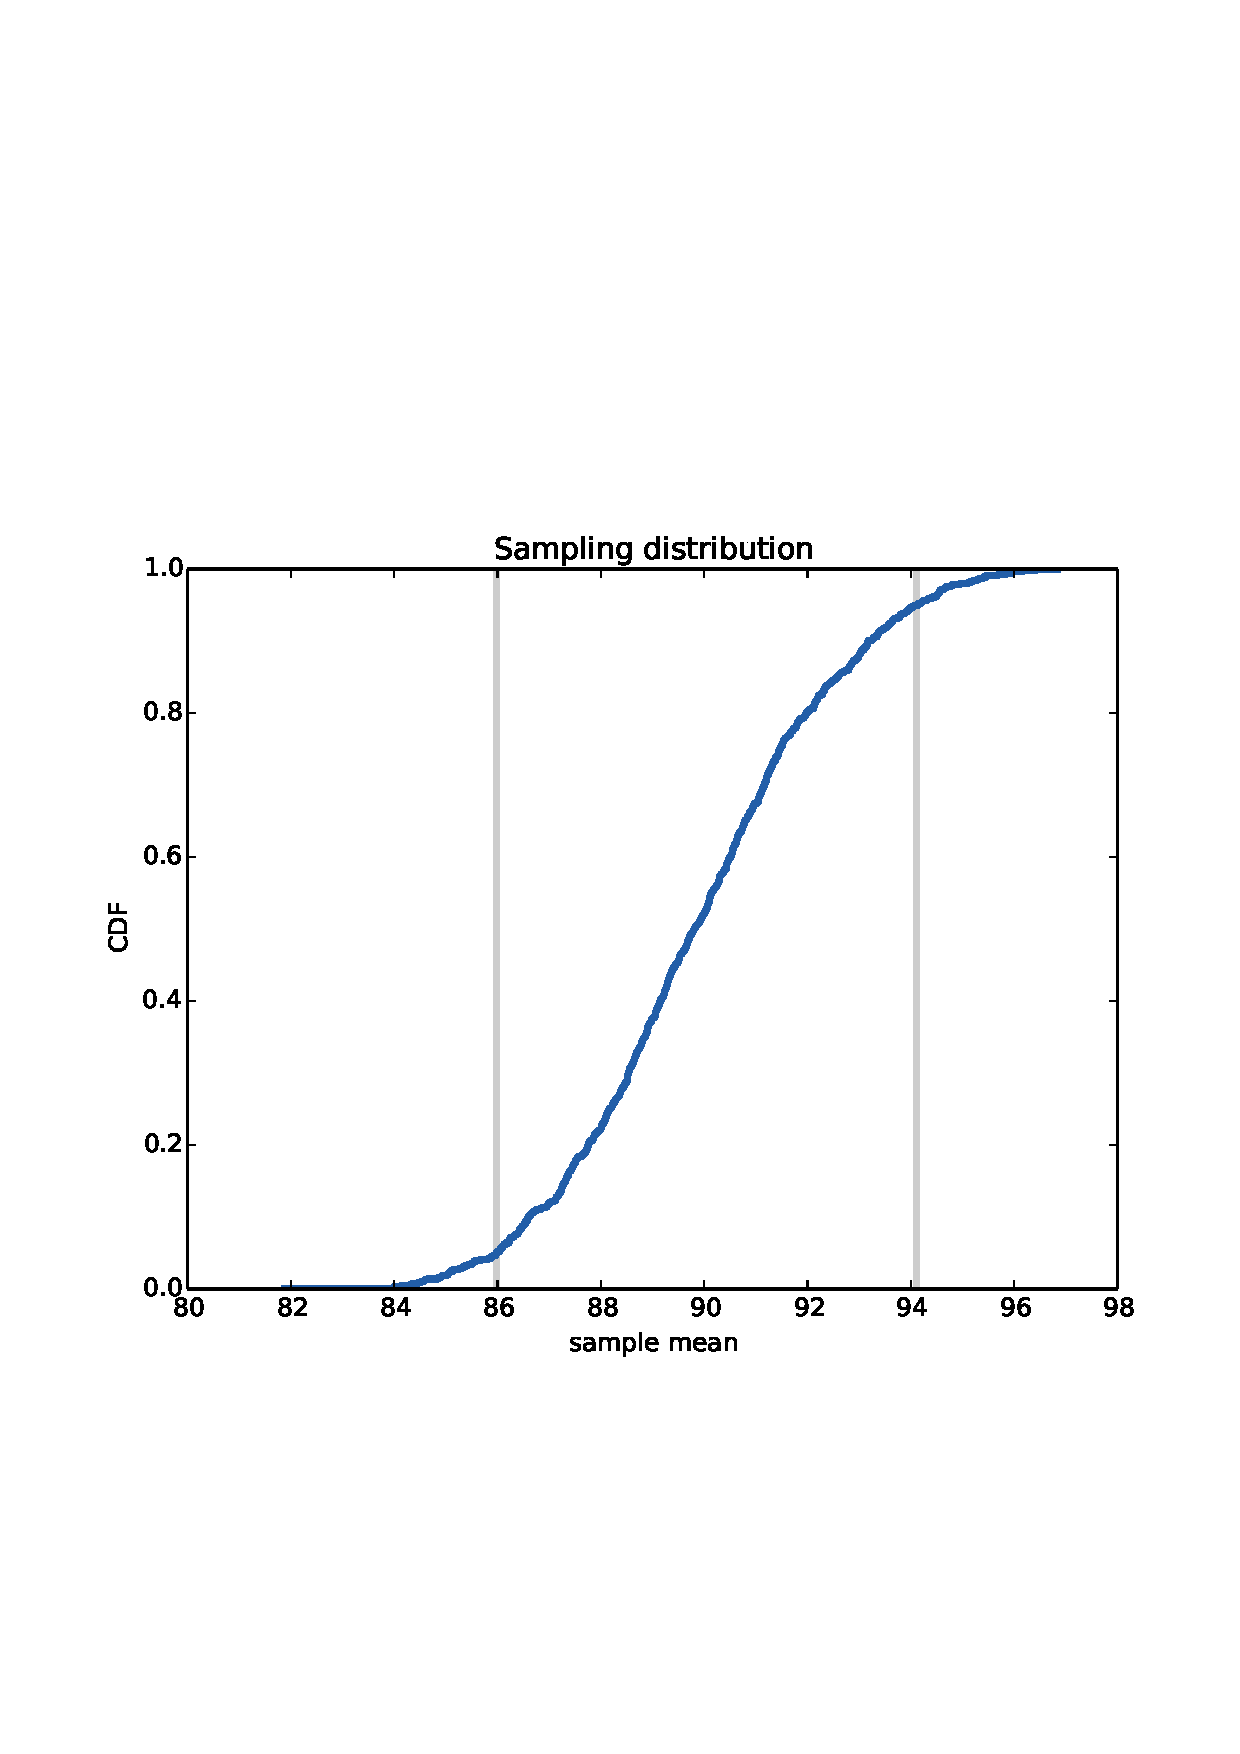
\includegraphics[height=2.5in]{figs/estimation1.pdf}}
\caption{신뢰구간과, $\xbar$ 표집분포.}
\label{estimation1}
\end{figure}

매번 반복할 때마다, 주어진 모수를 가진 정규분포에서 {\tt n}개 값을 골라 
표본 평균 {\tt xbar}를 계산한다. 1000번 모의시험하고 나서, 추정값 분포 {\tt cdf}를 계산한다. 결과가 그림 ~\ref{estimation1}에 나타나 있다.
분포를 추정값의 {\bf 표집 분포 (sampling distribution)}라고 부른다.
만약 반복해서 실험을 계속한다면, 추정값이 얼마나 변화하는지 보여준다.
\index{표집 분포 (sampling distribution)}

표집 분포 평균이 가정값(hypothetical value) $\mu$와 매우 가깝다.
따라서, 평균적으로 실험이 정답을 산출한다는 의미다.
1000회 반복한 후에는 가장 적은 값이 82 kg, 가장 큰 값이 98 kg이다.
이 범위가 함의하는 바는 추정값이 8 kg 만큼 차이가 있을 수 있다는 것이다.

표집 분포를 요약하는 두 가지 흔한 방법이 있다.

\begin{itemize}

\item {\bf 표준 오차 (Standard error SE)}는 평균적으로 추정값이 얼마나 차이가 있을지 측정하는 측도다. 각 모의 실험마다, 오차 $\xbar - \mu$를 계산하고 나서 누적평균제곱오차에 제곱근(root mean squared error, RMSE)을 씌워 계산한다. 상기 예제에서는 대략 2.5 kg이 된다.
\index{표준 오차 (standard error)}

\item {\bf 신뢰 구간 (confidence interval, CI)}은 표집 분포를 주어진 비율로 포함할 범위가 된다. 예를 들어, 신뢰 구간 90\%는 5번째부터 95번째 백분위수 범위가 된다. 상기 예제에서, 90\% CI는 $(86, 94)$ kg가 된다.
\index{신뢰 구간 (confidence interval)}
\index{표집 분포 (sampling distribution)}

\end{itemize}

표준 오차와 신뢰구간은 또한 혼동의 원천이기도 하다.

\begin{itemize}

\item 종종 표준 오차(standard error)와 표준편차(standard deviation)를 혼동한다. 표준 편차는 측정량에 내재한 변동성을 기술한다; 상기 예제에서, 고릴라 체중의 표준 편차는 7.5 kg이다. 표준 오차는 추정값에 내재한 변동성을 기술한다. 상기 예제에서, 표본 9 측정에 기반한 평균의 표준 오차는 2.5 kg 이다.

\index{고릴라 (gorilla)}
\index{표준 편차 (standard deviation)}

차이점을 기억하는 방법은, 표본 크기가 증가함에 따라, 
표준 오차는 점점 더 작아진다; 표준 편차는 그렇지 않다.
  
\item 90\% 확률로 실제 모수 $\mu$가 90\% 신뢰구간 내에 속한다고 생각하곤 한다. 슬프게도, 이것은 사실이 아니다.
이와 같은 주장을 하려고 한다면, 베이즈 방법(Bayesian method)을 사용해야 한다.(원저작자 책, {\it Think Bayes}을 참조).
\index{베이즈 통계 (Bayesian statistics)}

표집 분포는 다른 질문에 대한 답이다; 만약 실험을 반복한다면, 추정값이 얼마나 변화할 것인지 정보를 제시함으로써 추정값이 얼마나 신뢰할만한지 정보를 제공한다.
\index{표집 분포 (sampling distribution)}

\end{itemize}

신뢰 구간과 표준 오차는 표집 오차만 정량화한다는 것을 기억하는 것이 중요하다; 즉, 모집단 일부만 측정함으로써 생기는 오차.
표집 분포가 다른 오차를 설명하지는 않는다.
다른 오차는 표집 편의(sampling bias)와 측정 오차 (measurement error)가 포함되고 다음 절의 주제다. 

\section{표집 편의 (Sampling bias)}

자연보호구역에 고릴라 체중 대신에, 도시에 거주하고 있는 여성 평균 체중을 알고자 한다고 가정하자. 여성 대표 표본을 골라 체중을 측정하는 허가가 날 것 같지는 않다.

\index{고릴라 (gorilla)}
\index{성인 체중 (adult weight)}
\index{표집 편의 (sampling bias)}
\index{편의 (bias)!표집 (sampling)}
\index{측정 오차 (measurement error)}

간단한 대안은 ``전화 표집 (telephone sampling)''이 될 것이다; 
즉, 전화번호부에서 임의 번호를 골라, 전화하고, 성인 여성과 통화하여, 체중이 얼마인지 조사하는 것이다. 

\index{전화 표집 (telephone sampling)}
\index{난수 (random number)}

전화 표집은 분명한 한계가 있다.
예를 들어, 표본이 전화번호가 전화번호부에 등재된 사람으로 국한된다.
그래서 전화가 없는 사람(평균보다 더 가난할지 모르는 사람)과 전화번호부에 등재되지 않은 사람(훨씬 더 부자일 수 있는 사람)은 제외된다. 
또한, 낮 시간에 집으로 전화를 걸게 되면, 직장을 가진 사람이 표본에 있을 가능성은 줄어든다. 그리고 만약 전화에 응답한 사람만 표본으로 추출한다면, 전화를 공용으로 사용하는 사람을 표본으로 덜 추출할 것 같다.

수입, 실업, 가구 규모 같은 요인이 체중과 관련이 있다면(관련이 있을 듯하다.), 조사 결과가 어떻게든지 영향을 받을 수 있다. 이러한 문제를 {\bf 표집 편의 (sampling bias)}라고 부른다. 왜냐하면 표집과정(sampling process)의 한 특성이기 때문이다.
\index{표집 편의 (sampling bias)}

이러한 표집 과정은 또한 자기 선택(self-selection)에 취약한데 일종의 표집 편의다.
일부 사람은 질문에 대답을 거부한다. 그리고 만약 거부하는 경향이 체중과 관련된다면, 결과에도 영향을 줄 수 있다.
\index{자기 선택 (self-selection)}

마지막으로, 체중을 측정하기보다, 체중이 얼마인지 설문한다면, 결과가 정확하지 않을 수도 있다.
만약 실제 본인 체중에 불편하다면, 심지어 도움되는 응답자 조차도 체중을 올리거나 내릴지도 모른다. 그리고 모든 응답자가 도움이 되는 것은 아니다.
이와 같은 비정확성이 {\bf 측정 오차 (measurement error)} 사례가 된다.
\index{측정 오차 (measurement error)}

추정량을 보고할 때, 표집 오차를 정량화하기 위해서 표준 오차 혹은 신뢰구간, 혹은 모두 보고하는 것이 유용한다.
하지만, 표집 오차는 단지 오차의 단지 하나일 뿐이고, 종종 가장 큰 것이 아니라는 것을 기억하는 것이 중요하다.
\index{표준 오차 (standard error)}
\index{신뢰구간 (confidence interval)}


\section{지수분포 (Exponential distributions)}
\index{지수분포 (exponential distribution)}
\index{분포 (distribution)!지수 (exponential)}

한번더 추정 게임을 시도해보자. 
{\em 저자가 마음속에 분포를 하나 염두에 두고 있다.}
지수분포로, 다음에 표본이 있다.

{\tt [5.384, 4.493, 19.198, 2.790, 6.122, 12.844]}

상기 분포 모수 $\lambda$는 무엇이라고 생각하나요?

\index{모수 (parameter)}
\index{평균 (mean)}

\newcommand{\lamhat}{L}
\newcommand{\lamhatmed}{L_m}

일반적으로 지수분포 평균은 $1/\lambda$다. 그래서 역산해서 다음을 선택할 수 있다.
%
\[ \lamhat = 1 / \xbar\]
%
$\lamhat$은 $\lambda$의 추정량이다. 그리고 보통 다른 추정량과 다르다; 또한 최우추정량(maximum likelihood estimator)이다. (\url{http://wikipedia.org/wiki/Exponential_distribution#Maximum_likelihood} 참조).
그래서, 만약 정확하게 $\lambda$ 추측 확률을 극대화하려고 한다면, $\lamhat$이 나갈 방향이 된다.
\index{MLE}
\index{최우추정량 (maximum likelihood estimator)}

하지만, $\xbar$가 이상점이 존재하는 경우 강건하지 않다는 것을 알고 있다.
그래서, $\lamhat$도 동일한 문제를 작고 있다고 예상한다.
\index{강건성 (robust)}
\index{이상값 (outlier0}
\index{표본 중위수 (sample median)}

표본 중위수에 기반한 대안을 선택할 수 있다.
지수 분포 중위수는 $\ln(2) / \lambda$이다. 
다시 역산해서 계산하면, 추정량을 다음과 같이 정의한다.
%
\[ \lamhatmed = \ln(2) / m \]
%
여기서, $m$은 표본 중위수다.
\index{중위수 (median)}

이들 추정량 성능을 시험하기 위해서, 표집 과정을 모의 시험할 수 있다.

\begin{verbatim}
def Estimate3(n=7, m=1000):
    lam = 2

    means = []
    medians = []
    for _ in range(m):
        xs = np.random.exponential(1.0/lam, n)
        L = 1 / np.mean(xs)
        Lm = math.log(2) / thinkstats2.Median(xs)
        means.append(L)
        medians.append(Lm)

    print('rmse L', RMSE(means, lam))
    print('rmse Lm', RMSE(medians, lam))
    print('mean error L', MeanError(means, lam))
    print('mean error Lm', MeanError(medians, lam))
\end{verbatim}

$\lambda=2$로 실험을 하면, $L$ RMSE는 1.1 이 된다.
중위수 기반 추정량 $L_m$, RMSE는 1.8 이 된다.
실험으로부터 $L$ 이 MSE를 최소화했는지 분간할 수 없다.
하지만 적어도 $L_m$ 보다 더 좋은 듯 하다.
\index{MSE}
\index{RMSE}

슬프게도 두 추정량 모두 편의가 있다. $L$에 대해 평균 오차는 0.33; 
$L_m$에 대해 평균 오차는 0.45 다. 그리고 어느 것도 {\tt m}이 증가함에 따라 0 으로 수렴하지 않는다.
\index{편의 추정량 (biased estimator)}
\index{추정량 (estimator)!편의 (biased)}

$\xbar$는 분포 평균의 불편 추정량 $1 / \lambda$임이 밝혀졌다. 하지만,
$L$은 $\lambda$의 불편 추정량은 아니다.

\section{연습문제}

다음 연습문제에 대해서, {\tt estimation.py}을 복사해서 시작할 수 있다.
해답은 \verb"chap08soln.py" 파일에 나와있다.

\begin{exercise}

이번 장에서, $\mu$를 추정하는데 $\xbar$ 와 중위수를 사용했고,
$\xbar$가 MSE 하한을 산출함을 알아냈다.
또한, $\sigma$를 추정하는데 $S^2$ 와 $S_{n-1}^2$을 사용했고,
$S^2$은 편향되었고, $S_{n-1}^2$은 불편향임을 알아냈다.

유사한 실험을 실행해서, $\xbar$와 중위수가 $\mu$의 편향된 추정값임을 알아내라.
또한, $S^2$ 혹은 $S_{n-1}^2$ 가 MSE 하한을 산출하는지 검사하라.

\index{표본 평균}
\index{표본 중위수}
\index{추정량!편향된}

\end{exercise}


\begin{exercise}

모수 $\lambda=2$를 갖는 지수분포에서 표본 $n=10$ 개를 추출한다고 가정하자.
실험을 1000번 모의시험하고 추정값 $\lamhat$의 표본 분포를 도식화한다.
추정값의 표준오차와 90\% 신뢰구간을 계산하라.

\index{표준오차}
\index{신뢰구간}
\index{표본분포}

다른 $n$ 값을 갖는 실험을 반복하고, $n$ 값과 표준오차를 도식화한다.
\index{지수분포}
\index{분포!지수}


\end{exercise}


\begin{exercise}

하키와 축구같은 스포츠 게임에서 득점 사이 시간은 대체로 지수를 따른다.
그래서 게임에서 한 팀이 득점한 골을 관측함으로써 득점을 추정할 수 있다.
이 추정 과정은 득점 사이 시간을 표집하는 것과 약간 다르다. 
그래서 작동방법을 살펴보다.

\index{하키}
\index{축구}

게임당 골로 득점률 {\tt lam}을 인자로 받고,
전체 시간이 1 게임 경과할 때까지 득점사이 시간을 생성함으로서 게임을 
모의시험하고 나서, 득점한 점수를 반환하는 함수를 작성하라. 

많은 게임을 모의시험하고, {\tt lam} 추정값을 저장하고 나서
평균 오차와 RMSE를 계산하는 또다른 함수를 작성하라.

추정값을 이와 같은 방식으로 만드는 것이 편향됐을까?
추정값에 대한 표본분포와 90\% 신뢰구간을 도식화하시오.
표준오차는 얼마인가? 
{\tt lam} 값을 크게하면, 표집오차에 무슨일이 생길까?

\index{추정량!편향된}
\index{편향된 추정량}
\index{표준오차}
\index{신뢰구간}

\end{exercise}


\section{용어 사전}

\begin{itemize}

\item 추정 (estimation): 표본에서 분포 모수를 추정하는 과정.
\index{추정 (estimation)}

\item 추정량 (estimator): 모수를 추정하는데 사용되는 통계량.
\index{추정량 (estimator)}

\item 누적평균제곱오차 (mean squared error, MSE): 추정 오차 측도.
\index{누적평균제곱오차 (mean squared error)}
\index{MSE}

\item 제곱근 평균제곱오차 (root mean squared error, RMSE): 
MSE 제곱근으로 일반적인 오차 규모를 좀더 유의미하게 표현.
\index{누적평균제곱오차 (root mean squared error)}
\index{RMSE}

\item 최우추정량 (maximum likelihood estimator, MLE): 가장 올바를 것 같은 점추정값을 계산하는 추정량.
\index{MLE}
\index{최우추정량 (maximum likelihood estimator)}

\item (추정량의) 편의 (bias of an estimator): 반복되는 실험을 평균낼 때, 실제 모수 값보다 높은 혹은 낮은 추정량의 경향성. 
\index{편의 추정량 (biased estimator)}

\item 표집 오차 (sampling error): 
우연에 의한 변동과 한정된 표본 크기 때문에 추정값에 생기는 오차.
\index{점추정 (point estimation)}

\item 표집 편의 (sampling bias): 
모집단을 대표하지 못하는 표집 과정 때문에 추정값에 생기는 오차.
\index{표집 편의 (sampling bias)}

\item 측정 오차 (measurement error): 
데이터를 수집하고 기록하는 부정확성 때문에 추정값에 생기는 오차.
\index{측정 오차 (measurement error)}

\item 표집 분포 (sampling distribution): 
만약 실험을 많이 반복한다면 생기는 통계량 분포.
\index{표집 분포 (sampling distribution)}

\item 표본 오차 (standard error): 
추정값의 RMSE로 표집 오차 (하지만 다른 오차는 제외) 때문에 생기는 변동성을 정량화한다.
\index{표본 오차 (standard error)}

\item 신뢰구간 (confidence interval): 
만약 실험을 많이 반복하면 추정량 예상 범위를 표현하는 구간.
\index{신뢰구간 (confidence interval)} 
\index{구간 (interval)!신뢰 (confidence)}

\end{itemize}
